\clearpage
\Needspace{12\baselineskip}
\section{Low-resource protocols and diagnostic details}
\label{app:diagnostics}

The matched low-resource comparisons use the backbone and optimizer in
Table~\ref{tab:standard_shared_settings}, with the shorter schedule in
Table~\ref{tab:budget_protocol}. Exceptions and diagnostic evidence are
summarized below; full-budget results remain in the corresponding problems.

\begin{table}[htbp]
    \centering\footnotesize
    \begin{tabular}{@{}>{\raggedright\arraybackslash}p{0.16\textwidth}
        >{\raggedright\arraybackslash}p{0.43\textwidth}
        >{\raggedright\arraybackslash}p{0.34\textwidth}@{}}
        \toprule
        Check & Evidence & Interpretation / limitation \\
        \midrule
        Validation & Matched runs use fixed seed-42 windows. The earlier
        LR search drew random validation batches and consumed training RNG.
        & The old baseline (1.5966) and matched baseline (1.5879) are separate runs. \\
        \addlinespace
        LR selection & Last-ten validation means: 1.6629 / 1.6188 / 1.6333
        at peaks $5\times10^{-4}$ / $10^{-3}$ / $2\times10^{-3}$.
        & $10^{-3}$ is best among tested settings. Short screens use
        different cosine horizons. \\
        \addlinespace
        Large LR & Peak 0.3: training loss up to 305.5062; peak 0.5:
        up to 194.4761. See Figure~\ref{fig:lr_divergence}.
        & Finite spikes with recovery; no proven unbounded divergence
        or precise stability boundary. \\
        \addlinespace
        Batch / capacity & Batch 8/16 last-ten means: 1.5911/1.5937.
        Batch 1 had 2.68\,GiB system swap growth. Capacity probes passed
        at 48 and stopped at 56/64.
        & Timing includes validation/saving and memory pressure.
        Largest tested passing batch is not an absolute capacity limit. \\
        \addlinespace
        Parameter match & FFN weights/block: SwiGLU 2,064,384;
        SiLU 2,097,152. Overall SiLU parameter count is 0.58\% higher.
        & Approximate capacity match; all rankings use one seed and
        mostly fixed LR settings. \\
        \bottomrule
    \end{tabular}
    \caption{Diagnostic evidence and limits on interpreting the low-resource comparisons.}
    \label{tab:diagnostic_summary}
\end{table}

\textbf{Why lower the no-RMSNorm learning rate?}
An earlier no-RMSNorm probe at peak $10^{-3}$ reached validation losses
7.4620 and 2125.2192 at updates 300/400, then recovered to 2.4755 at 1,000.
Peaks $3\times10^{-4}$ and $5\times10^{-4}$ were screened with the long
schedule; the latter won all ten evaluations (final 2.4873 versus 2.5967).
Figure~\ref{fig:no_rmsnorm_stability} shows the first 1,000 updates of the
subsequent complete run at the selected peak, rather than the earlier probes.

\begin{figure}[htbp]
    \centering
    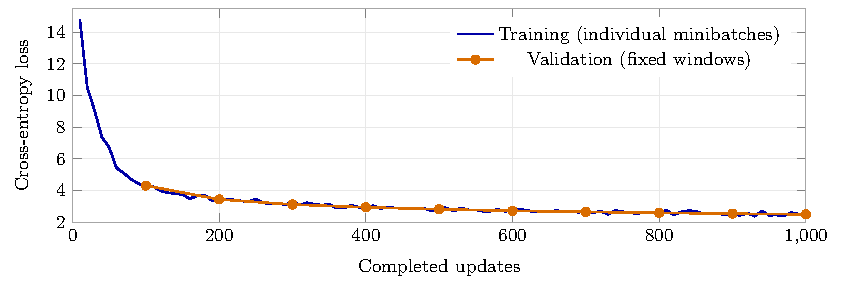
\includegraphics[width=0.88\textwidth]{figures/no_rmsnorm_stability.pdf}
    \caption{Early training without RMSNorm at peak LR $5\times10^{-4}$.
    All 100 logged minibatch losses and ten fixed-window validation losses
    through update 1,000 are shown without smoothing; validation ends at
    2.4872. This supports early stability at the selected setting, not LR
    optimality or a controlled comparison with the earlier probes.}
    \label{fig:no_rmsnorm_stability}
\end{figure}
\FloatBarrier

\textbf{Comparison boundaries.}
Batch schedules scale inversely with batch size to match tokens (batch 48
uses 0.01\% fewer); fixed AdamW settings still change moment timescales and
decay per token. The batch-32 result uses a fresh complete rerun after an
initial memory-pressure stop. The no-RMSNorm result changes LR as well as
architecture. Standard runs extend both budget and LR schedule; TinyStories
also changes backend. These runs do not establish significance, long-budget
ablation rankings, or generally optimal generation temperatures.
